%-synctex=1 -undump=pdflatex %ProjectDir%\%ProjectName%.tex --c-style-errors --interaction=batchmode --aux-directory=temp
\documentclass[12pt,a4paper,pdftex]{report}
\usepackage[utf8]{inputenc}
\usepackage[T1]{fontenc}

\usepackage[nohyperlinks]{acronym}
\usepackage[unicode,breaklinks=true,hypertexnames=false]{hyperref}
\usepackage{pdfpages} 
\usepackage{enumitem}
\usepackage{tabularx}

\usepackage{cmap}

\usepackage{lmodern}
\usepackage{textcomp}

%\usepackage{circuitikz}
\usepackage{tikz}
\usepackage{pgfplots}
\usepackage{amsmath}
\usetikzlibrary{calc,arrows,positioning,decorations,trees,chains}
\usepgfplotslibrary{patchplots,groupplots,units}

\usepackage{pgfplotstable}
\usepackage{verbatim}
\usepackage{array}
\usepackage{amssymb}
\usepackage{amsthm}
\usepackage{siunitx}





%%%%%%%%%%%%%%%%%%%%%%%%%%%%%%%%%%%%%%%%%%%%%%%%%%%%%%%%%%%%%%%%%%%%%%%
%%%%%%%%%%%%%%%%%%%%%%%%%%%%%%%%%%%%%%%%%%%%%%%%%%%%%%%%%%%%%%%%%%%%%%%
\begin{document}

\part{The principle of operation}

\part{The hardware}

\part{The console app}

\part{The GUI application}

\section{Introduction}

\begin{figure}[ht!]
	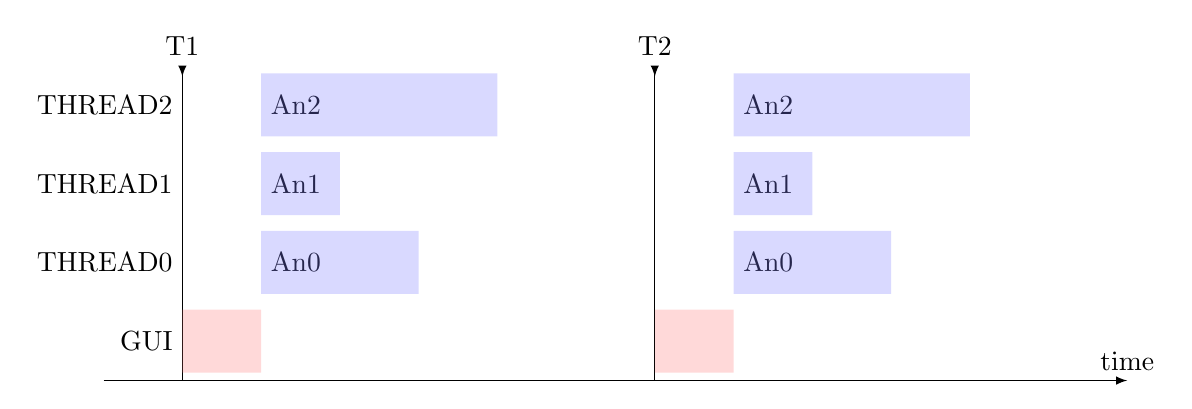
\begin{tikzpicture}[>=latex]
		\draw[->] (0,0) -- ++(13,0) node[above] {time};
		\draw[-<] (1,0) -- ++(0,4) node[above] {T1};
		\draw[-<] (7,0) -- ++(0,4) node[above] {T2};
		\path 
			(1,0.5) coordinate (gui-0) node[left] {GUI}
			++(0,1) coordinate (t0) node[left] {THREAD0}
			++(0,1) coordinate (t1) node[left] {THREAD1}
			++(0,1) coordinate (t2) node[left] {THREAD2}
			(1,0.5) coordinate (gui-0s)
			(2,0.5) coordinate (gui-0e)
			++(0,1) coordinate (t0-0s) node[right] {An0}
			++(0,1) coordinate (t1-0s) node[right] {An1}
			++(0,1) coordinate (t2-0s) node[right] {An2}
			(4,1.5) coordinate (t0-0e)
			(3,2.5) coordinate (t1-0e)
			(5,3.5) coordinate (t2-0e)
			([xshift=6cm]gui-0s) coordinate (gui-1s)
			([xshift=6cm]gui-0e) coordinate (gui-1e)
			([xshift=6cm]t0-0s) coordinate (t0-1s) node[right] {An0}
			([xshift=6cm]t1-0s) coordinate (t1-1s) node[right] {An1}
			([xshift=6cm]t2-0s) coordinate (t2-1s) node[right] {An2}
			([xshift=6cm]t0-0e) coordinate (t0-1e)
			([xshift=6cm]t1-0e) coordinate (t1-1e)
			([xshift=6cm]t2-0e) coordinate (t2-1e)
			;
		\fill[red!50,opacity=0.3]
			([yshift=-0.4cm]gui-0s) rectangle ([yshift=0.4cm]gui-0e)
			([yshift=-0.4cm]gui-1s) rectangle ([yshift=0.4cm]gui-1e)
			;
		\fill[blue!50,opacity=0.3]
			([yshift=-0.4cm]t0-0s) rectangle ([yshift=0.4cm]t0-0e)
			([yshift=-0.4cm]t1-0s) rectangle ([yshift=0.4cm]t1-0e)
			([yshift=-0.4cm]t2-0s) rectangle ([yshift=0.4cm]t2-0e)
			([yshift=-0.4cm]t0-1s) rectangle ([yshift=0.4cm]t0-1e)
			([yshift=-0.4cm]t1-1s) rectangle ([yshift=0.4cm]t1-1e)
			([yshift=-0.4cm]t2-1s) rectangle ([yshift=0.4cm]t2-1e)
			;
	\end{tikzpicture}
	\caption{The multithreading nature of Analyzer data flow}
\end{figure}

GUI is updating displays with results from previous analyzer's run, and harvesting package for the next analyzer run.

\begin{figure}[ht!]
	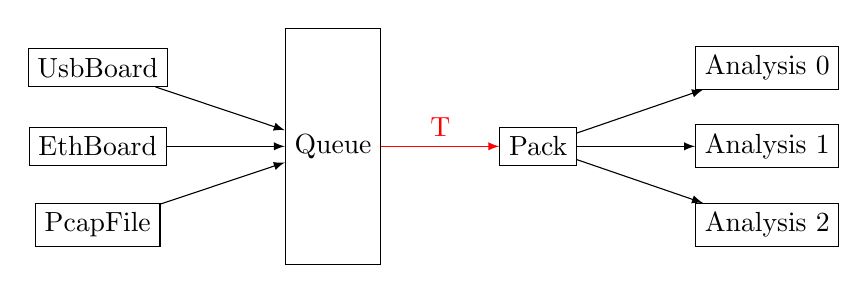
\begin{tikzpicture}[>=latex]
		\node[draw,rectangle,minimum height=3cm] (queue) {Queue};
		\node[draw,rectangle,right=1.5cm of queue] (pack) {Pack};
		\node[draw,rectangle,left=1.5cm of queue] (eth) {EthBoard};
		\node[draw,rectangle,above of=eth] (usb) {UsbBoard};
		\node[draw,rectangle,below of=eth] (pcap) {PcapFile};
		\node[draw,rectangle,right=1.5cm of pack] (analysis1) {Analysis 1};
		\node[draw,rectangle,above of=analysis1] (analysis0) {Analysis 0};
		\node[draw,rectangle,below of=analysis1] (analysis2) {Analysis 2};
		
		\path
			(usb) edge[->] (queue)
			(eth) edge[->] (queue)
			(pcap) edge[->] (queue)
			(queue) edge[->,red] node[above] {T} (pack)
			(pack)
				edge[->] (analysis0)
				edge[->] (analysis1)
				edge[->] (analysis2)
			;
	\end{tikzpicture}
	\caption{The data flow through analysis}
\end{figure}

Queue is ConcurrentQueue, so all boards/files can write to it from threads.

The Pack is only array, so it is thread safe to read it. It is constructed
periodically from the main GUI thread with period T from data in queue taken
from previous grab, and possibly filtered in this phase (needs revision).

Each analysis runs its own thread, producing intermediate and cumulative results.

The results are presented on the displays just before the new analysis stage runs.

If any of the analysis threads is still running during period T, all actions of
this period are skipped with leaving data in queue.

\end{document}
